\chapter{Introduction}
Application Programming Interfaces, commonly known as APIs, are used to express a software component in terms of its operations, inputs, outputs, and their types\footnote{\url{https://en.wikipedia.org/wiki/Application_programming_interface}}. Robillard defines an API as follows: An API is the interface to implement functionality that developers can access to perform various tasks \cite{Robillard_a_field_study, Robillard_what_makes}. APIs enable multiple software components to interact with each other.

REST APIs are a type of APIs that are used to integrate software components using web technologies. Fielding defined Representational State Transfer or REST as an architectural style for developing distributed hypermedia systems \cite{Fielding_rest}. For example, GitHub, an online code repostory hosting tool, has a REST API that can be used by third-party applications to integrate with GitHub features. The GitHub REST API\footnote{\url{https://developer.github.com/v3/repos/\#create}} has a resource called \texttt{Repository} to denote a code repository that can be identified by the URL \url{/user/repos}. To create a new \texttt{Repository} for a user, the GitHub API can be invoked via HTTP $POST$ at \url{/user/repos} using the following JSON representation of a \texttt{Repository}:

\begin{verbatim}
{
  "name": "Hello-World",
  "description": "This is your first repository",
  "homepage": "https://github.com",
  "private": false,
  "has_issues": true,
  "has_wiki": true,
  "has_downloads": true
}
\end{verbatim}

In today's world of technology, REST APIs have become ubiquitous and the primary choice for integrating Internet enabled applications due to its simplicity and similarity with HTTP \cite{mangler2010origin}. For example, a real estate listing website uses a REST API to collect ``walk score'' and another REST API to show a map view of a property listing. By incorporating the map and walk score using REST APIs, the real estate listng site provides important information to their users. Most REST APIs, including these two examples, are often documented manually or using custom implemented tools specific to the APIs that are not publicly available. This requires effort to generate and maintain the documentation of REST APIs over time since there is a lack of reusable tool support.

Previous research in the area of API usability mostly focused on local APIs such as Java libraries. Researchers identified the documentation of APIs as both the primary source of information as well as the key obstacle for API usability \cite{Robillard_what_makes}. Hence the quality of the API documentation plays an important role in API usability. To this regard, researchers have identified the qualities of ``good API documentation'' as follows: complete, correct, includes thorough explanations and code examples, provides consistent presentation and organization \cite{Robillard_what_makes,Myers_study}. Today, there are several tools such as Javadoc\footnote{\url{http://www.oracle.com/technetwork/java/javase/documentation/index-jsp-135444.html}}, UsETeC \cite{zhu2014mining}, Jadeite \cite{Jadeite}, APIMiner \cite{montandon2013documenting}, Roast \cite{Hoffman_api_documentation} that can be used to document local APIs with the aforementioned qualities .

While there are overlaps between the documentation requirements of local and REST APIs, there are significant requirements that are unique to each. The documentation of most local APIs contain a structrual definition of the API classses and methods. API usage examples for local APIs are documented using the same programming language of the API. On the other hand, REST APIs are defined using HTTP specific parameters such as API endpoints, query parameters, HTTP headers and body. REST API clients can use any programming language agnostic to the API implementation language. Due to such structural and implemenation differences between local and REST APIs, the existing technique and tools for local API documentation cannot be readily used to generate REST API documentation.

\begin{figure}[htb]
  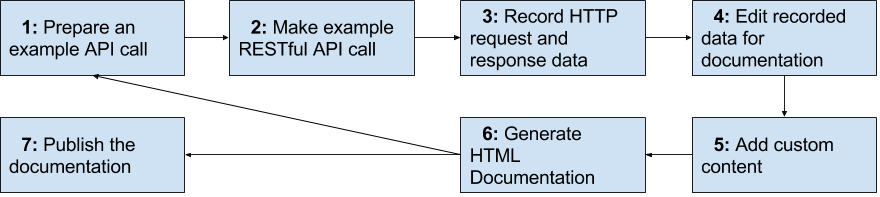
\includegraphics[width=\linewidth]{manual_workflow.png}
  \caption{Manual REST API Documentation Steps}
  \label{fig:manual}
\end{figure}

Currently, the process of documenting REST APIs is largely manual. Conceptually, the high level steps involved in the manual process can be identified as shown in Figure \ref{fig:manual}. These steps S1-S7 can be described as follows:

\begin{itemize}
  \item S1 - API developer prepares an example API with the required HTTP parameters and request body.
  \item S2 - API developer uses a REST API client to make the example API call.
  \item S3 - the API developer records the HTTP data.
  \item S4 - API developer then edits the recorded data so that only relevant content is selected for documentation.
  \item S5 - API developers use any custom content to describe the API example.
  \item S6 - API developers combine the custom content with the edited content from the HTTP traffic into HTML to publish to the web.
  \item S7 - API developer adds custom overview information to explain API concepts and general rules, and publishes the final documentation so other developers can learn the API
\end{itemize}

The steps S1-S6 are repeated for every API action that needs to be documented, and S1-S7 need to repeated for every version of the REST API as it evolves. As depicted here, this manual process can be both time consuming and error-prone.

The overarching goal of my research was to improve the current state of REST API documentation process by automating the repeating manual steps in the aforementioned workflow. More specifically, I aimed to solve the following research goals:

\begin{itemize}
  \item G1: To identify a set of REST API documentation requirements.
  \item G2: To develop and evaluate a technique to overcome the commonly observed but unresolved challenges related to REST API documentation.
\end{itemize}

To reach these goals, I have followed a strategy involving five smaller research projects as follows. The first research project, related to G1, is described in Chapter~\ref{chapter:case_study}, where I discuss a case study to summarize the state of existing literature and industry practices related to the versioning, documentation, and change communication patterns of evolving Web APIs \cite{sohan2015case}. The results are based on a study of nine industrical APIs selected based on their diverse application domains, maturity level, and popularity including both open and closed source implementations. The primary findings from this study are as follows: Web APIs evolve frequently, often several times a week, including both compatible and incompatible API changes, using manual or bespoke methods to version, document, and communicate the changes as they evolve. I found a lack of reusable techniques in the existing literature to automatically generate and maintain the documentation of multi-version evolving REST APIs with usage examples. I persued further research to solve this problem as discussed in the following paragraphs.

In Chapter~\ref{chapter:spy_rest}, I discuss my second research project, related to both G1 and G2, where I derived a set of REST API documentation requirements and proposed a new technique to satisfy the requirements. Here, I present the following list of REST API documentation requirements by studying the literature and applying the findings from Chapter~\ref{chapter:case_study}: 1) automated, 2) example based, 3) executable, 4) version aware, 5) customizable, 6) reusable, and 7) collaborative \cite{sohan2015spyrest}. I discuss the available REST API documentation techniques that require repeatitive manual efforts to generate and maintain custom formatted API descriptions that fail to satisfy these requirements. I present, SpyREST, a novel technique to intercept example REST API calls using an HTTP proxy server to collect and autmatically synthesize API traffic to generate and update API documentation to satisfy the aforementioned requirements. The primary advantage of the presented technique is that the documentation is generated from executable code. As a result, a continuously updated REST API documentation with realistic usage examples is achievable with a reduced manual effort.

I present my third research project, related to G2, in Chapter~\ref{chapter:demo_paper}, where I present a prototype implementation of the aformentioned technique \cite{sohan2015spyrest_tool}. Here, I demonstrate a reusable tool and compare it against the existing REST API documentation tools that rely on custom API description languages. In this prototype implementation, I discuss the process that transforms a number of example HTTP requests and responses into a usable REST API documentation. I also present an example where automated test code is used to generate and maintain a continuously updated REST API documentation using the developed tool.

I discuss my fourth research project, related to G2, involving an industrial evaluation of the proposed technique and the tool in Chapter~\ref{chapter:cisco_study} \cite{sohan_cisco}. The evaluation is carried out based on the data collected from an eighteen month of production use of SpyREST at Cisco, my current employer. From the study I found that it is feasible to use the proposed interception technique and automated tests to document evolving REST APIs satisfying the previously presented REST API documentation requirements. Automated always-updated REST API documentation was found to help establish a quick feedback cycle among the stakeholders. I also discuss several refinements and limitations of the proposed technique based on the lessons learned from this case study.


I present my fifth research project, related to G2, in Chapter~\ref{chapter:controlled_study}, where I discuss a controlled study to undestand the impact of usage examples in API documentation on REST API client developers \cite{sohan_vlhcc}. I recruited a total of 26 professional software engineers with REST API experience for this study. I mapped the participants into two groups and introduced usage examples as the control variable. I enhanced an existing REST API documentation with new usage examples. I gave the enhanced API documentation to participants from one of the study groups. I found that participants using the original documentation without usage examples faced common obstacles related to using appropriate data types, data formats, and required elements in the HTTP headers and request body. I observed that providing usage examples with data taken from API test code reduces the obstacles and improves API client developer success rate, reduces required trial attempts, and improves satisfaction ratings. The findings from this study provides an empirical evidence that by using the proposed technique of generating REST API documentation from API test code can help API client developers to achive a higher level of success with a reduced effort.

In summary, this thesis makes the following key contributions to the body of research in software engineering:

\begin{enumerate}
  \item A list of REST API documentation requirements derived from the existing literature and the current state of industry practices to be used as a guideline by practitioners and researchers.
  \item SpyREST, a novel technique and a reusable tool that uses interception to automatically generate and maintain evolving REST API documentation with usage examples from executable code.
  \item An industrial evaluation of SpyREST to demonstrate the feasibility of the proposed technique that practitioners can follow to improve their REST API documentation experience.
  \item An empricial evidence showing the common obstacles faced by REST API client developers that can be reduced with usage examples to help the prioritization of REST API documentation efforts.
\end{enumerate}

\bibliographystyle{IEEEtran}
\bibliography{IEEEabrv,references}


